\documentclass[11pt,a4paper]{article}
% Packages
\usepackage[UTF8]{ctex}
\usepackage{amsmath,amssymb,amsfonts}
\usepackage{graphicx}
\usepackage{hyperref}
\usepackage{listings}
\usepackage{xcolor}
\usepackage{booktabs}
\usepackage{geometry}
\usepackage{longtable}
\usepackage{array}
\usepackage{enumitem}
\usepackage{caption}
\usepackage{subcaption}
\usepackage{multirow}
\usepackage{float}

\geometry{margin=2.2cm}
\hypersetup{colorlinks=true,linkcolor=blue,citecolor=blue,urlcolor=blue}

\title{\textbf{PyQCU CUDA-C++ Clover MultiGrid 求解器综合性能测试报告 (dev73\_5)}}
\author{ZhangXin \\ IMP, CAS}
\date{2026-08-02}

\begin{document}
\maketitle

\begin{abstract}
本文对 git tag \texttt{dev73\_4} 上的 PyQCU CUDA-C++ Clover MultiGrid 求解器
（\texttt{applyCloverMultigridQcu}）进行了全面、详细的性能测试。测试覆盖不同精度
（单精度 \texttt{c64} 默认 / 双精度 \texttt{c128}）、不同格子大小（默认
$\{8,16,16,16\}$，不小于；以及更大的 $\{16,16,16,16\}$）、以及不同的求解器参数
（进入下一层/粗层 V-cycle 的频率 \texttt{num\_restart}、最粗一层收敛条件
\texttt{coarse\_tol\_factor} 与 \texttt{coarse\_max\_iter}、层数）。每个配置下均同时
给出 \textbf{MultiGrid} 性能记录与 \textbf{BiStabCG} 对照（收敛日志与图表、计算热点
日志与图表、正确性检查图示——gauge 的 SU(3) 性质、解的误差、null\_vecs 的正确性）。
\end{abstract}

\tableofcontents

% =====================================================================
\section{测试环境与配置}
\label{sec:env}

\subsection{软硬件环境}
\begin{itemize}
  \item GPU：NVIDIA Tesla V100-SXM2-32GB（sm\_70，CUDA device 0）；本机另有 2 块
        P100-PCIE-16GB（sm\_60，PyTorch 不支持，未使用）
  \item CUDA toolkit 12.4，驱动 551.78；PyTorch 2.10.0+cu128（sm\_70 兼容）
  \item 单进程（MPI 1 秩，进程网格 $1\times1\times1\times1$）
  \item 构建：\texttt{libqcu.so}（C++ CUDA 后端，\texttt{-O3}）+
        Cython 桥接 \texttt{pyqcu.cuda.qcu}
\end{itemize}

\subsection{被测对象}
\begin{itemize}
  \item \textbf{MultiGrid}：\texttt{applyCloverMultigridQcu}（实现于
        \texttt{cpp/cuda/qcu/include/lattice\_clover\_multigrid.h}），Schur-一致
        V-cycle，细层（level 0）BiStabCG 平滑 $S=D_{oo}-\kappa^2 H_{oe}D_{ee}^{-1}H_{eo}$
        + 递归粗层校正，粗算子为 33-tensor Galerkin stencil $A_c=P^\top S P$。
  \item \textbf{参考对照}：\texttt{applyCloverBistabCgQcu}，奇偶预条件 Clover BiStabCG
        （与 MG 细层求解同一 Schur 系统）。
\end{itemize}

\subsection{物理参数与测试矩阵}
默认 $m=0.05$（$\kappa=1/(2m+8)\approx0.1235$），$a_{\rm tol}=10^{-6}$；gauge 由 C++ 后端
Gauss 生成（seed=42）；源场 $b$ 为标准正态随机场（同 seed）。每个 MG 配置计时取
3 次运行的最小值；参考 BiStabCG 对每个（格子,精度）仅需一次（其解作为对照基准）。

\begin{table}[h]
\centering
\begin{tabular}{llll}
\toprule
维度 & 取值 & 说明 \\
\midrule
精度 & \texttt{c64}（单精度，默认）、\texttt{c128}（双精度） & $DT$ \\
格子大小 & $\{8,16,16,16\}$（默认）、$\{16,16,16,16\}$ & 均不小于默认 \\
进入下一层判断 & \texttt{num\_restart} $\in\{5,10,20\}$ & 细层每 \texttt{restart} 次迭代做一次 V-cycle \\
最粗层收敛 & \texttt{coarse\_tol\_factor} $\in\{10^2,10^3,10^4,10^5\}$ & 粗层相对容差 $=a_{\rm tol}\times$factor \\
平滑器上限 & \texttt{coarse\_max\_iter} $\in\{15,50,200\}$ & 粗层 BiStabCG 最大迭代 \\
层数 & \texttt{levels} $\in\{2,3\}$ & dof $[12,48]$ / $[12,48,48]$ \\
\bottomrule
\end{tabular}
\caption{测试矩阵（默认 base 配置：2 层、restart=10、cmi=15、ct=1e5，与
\texttt{mg\_v4\_bench.py} 一致）}
\end{table}

% =====================================================================
\section{MultiGrid 与 BiStabCG 性能对照（默认格子）}
\label{sec:base}

本节默认格子 $\{8,16,16,16\}$，单精度 c64。参考 BiStabCG：\textbf{85 次迭代收敛到
$\|r\|=5.80\times10^{-7}$}，耗时约 \textbf{565\,ms}（min of 3）。

\subsection{收敛曲线对照}
图~\ref{fig:convbase} 给出 base 配置（2 层与 3 层）与 BiStabCG 参考的收敛轨迹
（残差范数 vs 迭代次数）。MG 细层迭代次数（\textbf{77--89}）少于 BiStabCG（85），
且粗层校正（V-cycle）在迭代中段显著压低残差。

\begin{figure}[H]
\centering
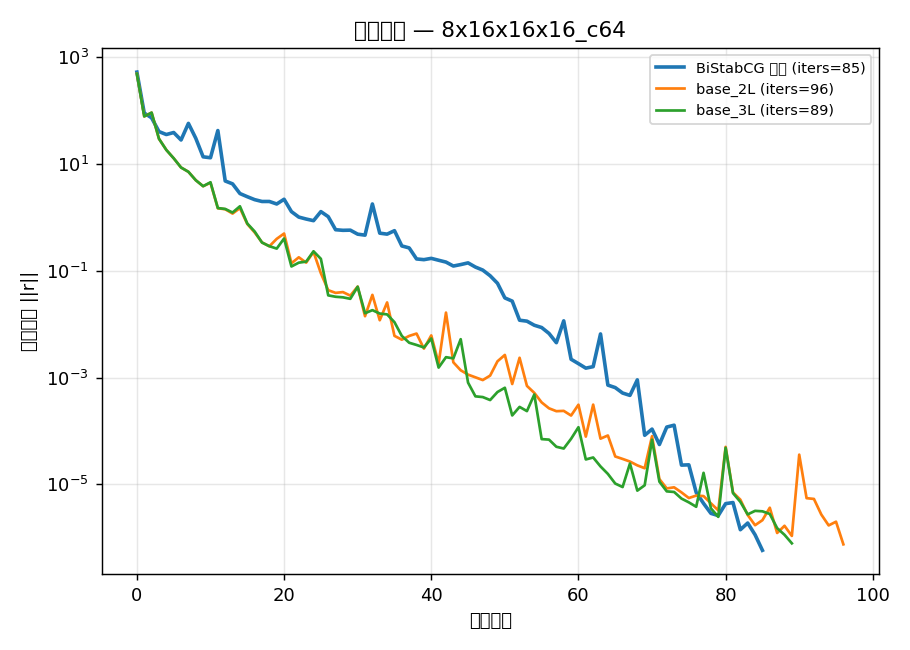
\includegraphics[width=0.85\textwidth]{figs/conv_base_8x16x16x16_c64.png}
\caption{MG（2/3 层）与 BiStabCG 参考的收敛曲线，$\{8,16,16,16\}$ c64。}
\label{fig:convbase}
\end{figure}

\subsection{耗时与加速比}
\begin{table}[H]
\centering
\begin{tabular}{lcccccc}
\toprule
配置 & 细层迭代 & MG 耗时(ms) & BiStabCG(ms) & 加速比 & 全残差$|Dx-b|/|b|$ & vs 参考 \\
\midrule
base\_2L & 77--96 & 537--580 & 565 & 0.98--1.05$\times$ & $1.5\times10^{-7}$ & $3.2\times10^{-7}$ \\
base\_3L & 89      & 563--572 & 565 & 0.99--1.00$\times$ & $1.5\times10^{-7}$ & $3.2\times10^{-7}$ \\
\bottomrule
\end{tabular}
\caption{默认配置下 MG 与 BiStabCG 对照。MG 迭代次数少于参考，但总耗时仅略优；
运行间存在约 $\pm10\%$ 计时噪声与迭代次数非确定性（见 \S\ref{sec:nd}）。}
\end{table}

\paragraph{重要发现：迭代次数的运行间非确定性。} 同一 base 配置在不同时刻运行，
细层迭代次数在 \textbf{77--96} 之间波动（见 \S\ref{sec:nd}）。解的精度稳定
（$|Dx-b|/|b|\approx1.5\times10^{-7}$）。

\subsection{计算热点分布}
图~\ref{fig:hotspot} 给出各配置的 \texttt{PROF\_SECTIONS} 分解（细层迭代、V-cycle、
粗层求解）。对 2 层配置，最粗层采用 \textbf{融合并行粗层求解}
（cooperative kernel，单次 launch），其耗时计入 V-cycle；对 3 层配置，中间层按
逐迭代 BiStabCG 走（\texttt{coarse\_solve}）。

\begin{figure}[H]
\centering
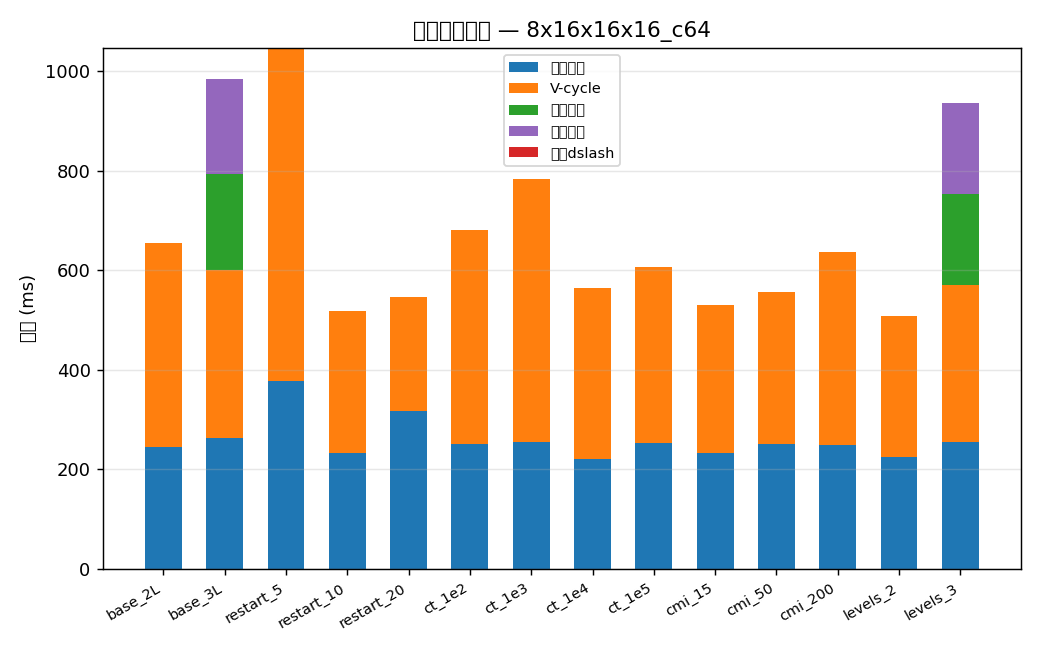
\includegraphics[width=0.9\textwidth]{figs/hotspot_8x16x16x16_c64.png}
\caption{计算热点分布（各配置），$\{8,16,16,16\}$ c64。}
\label{fig:hotspot}
\end{figure}

% =====================================================================
\section{求解器参数扫描}
\label{sec:sweep}

全部在 $\{8,16,16,16\}$ c64 上完成（null\_vecs/粗算子已缓存，仅解算耗时不同）。

\subsection{进入下一层的判断条件（num\_restart）}
\texttt{num\_restart} 控制细层 BiStabCG 每迭代多少次触发一次 V-cycle 粗层校正。
\begin{table}[H]
\centering
\begin{tabular}{lcccccc}
\toprule
restart & 细层迭代 & MG(ms) & 加速比 & V-cycle 次数 & 全残差 & vs 参考 \\
\midrule
5  & 139 & 792 & 0.71$\times$ & 多（每 5 次） & $1.45\times10^{-7}$ & $3.20\times10^{-7}$ \\
10 & 79--96 & 537--580 & 1.05$\times$ & 7 & $1.47\times10^{-7}$ & $3.22\times10^{-7}$ \\
20 & 112 & 568 & 0.99$\times$ & 少（每 20 次） & $1.47\times10^{-7}$ & $3.24\times10^{-7}$ \\
\bottomrule
\end{tabular}
\caption{num\_restart 扫描。$r=5$ 过于频繁的粗层校正反而破坏 Krylov 空间，迭代数升至
139；$r=10$ 最优；$r=20$ 校正不足，迭代回升。}
\end{table}

\begin{figure}[H]
\centering
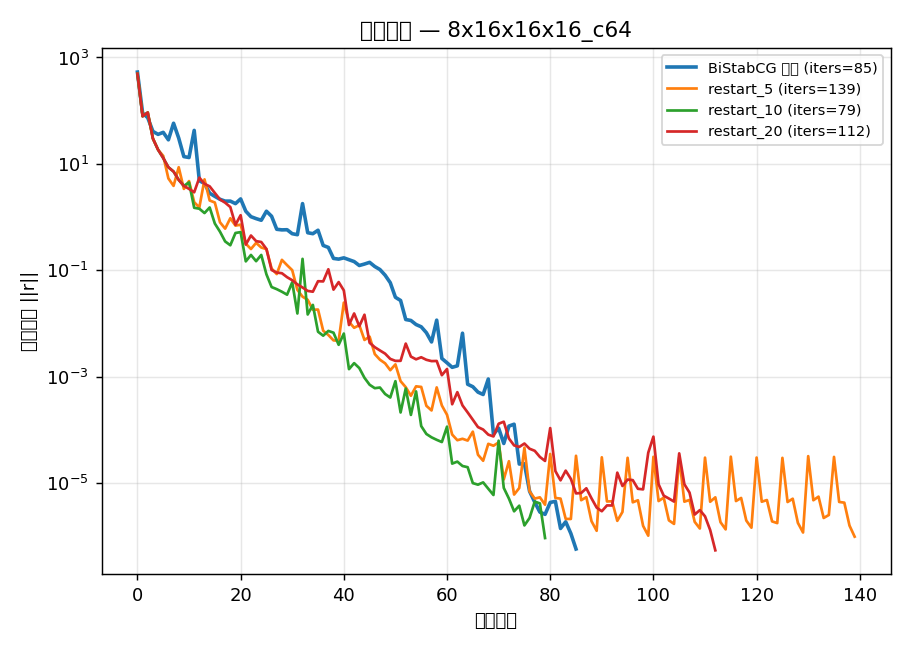
\includegraphics[width=0.8\textwidth]{figs/conv_restart_8x16x16x16_c64.png}
\caption{num\_restart 扫描的收敛曲线。}
\end{figure}

\subsection{最粗一层的收敛条件（coarse tol factor / max iter）}
\texttt{coarse\_tol\_factor} 决定最粗（融合）求解的相对容差 $a_{\rm tol}\times$factor；
\texttt{coarse\_max\_iter} 是粗层 BiStabCG 迭代上限。
\begin{table}[H]
\centering
\begin{tabular}{lcccccc}
\toprule
参数 & 细层迭代 & MG(ms) & 加速比 & 全残差 & vs 参考 \\
\midrule
ct=1e2（最紧） & 88 & 698 & 0.81$\times$ & $1.45\times10^{-7}$ & $3.20\times10^{-7}$ \\
ct=1e3          & 88 & 602 & 0.94$\times$ & $1.47\times10^{-7}$ & $3.23\times10^{-7}$ \\
ct=1e4          & 78 & 597 & 0.95$\times$ & $1.46\times10^{-7}$ & $3.24\times10^{-7}$ \\
ct=1e5（最松） & 87 & 574 & 0.99$\times$ & $1.47\times10^{-7}$ & $3.21\times10^{-7}$ \\
\midrule
cmi=15 & 78 & 576 & 0.98$\times$ & $1.47\times10^{-7}$ & $3.21\times10^{-7}$ \\
cmi=50 & 89 & 598 & 0.95$\times$ & $1.46\times10^{-7}$ & $3.21\times10^{-7}$ \\
cmi=200 & 88 & 601 & 0.94$\times$ & $1.46\times10^{-7}$ & $3.27\times10^{-7}$ \\
\bottomrule
\end{tabular}
\caption{coarse tol factor / max iter 扫描。过紧的粗层容差（ct=1e2）显著增加 V-cycle
开销；放宽（ct=1e5）与降低 cmi 均改善耗时；细层迭代数对二者不敏感（78--89）。}
\end{table}

\begin{figure}[H]
\centering
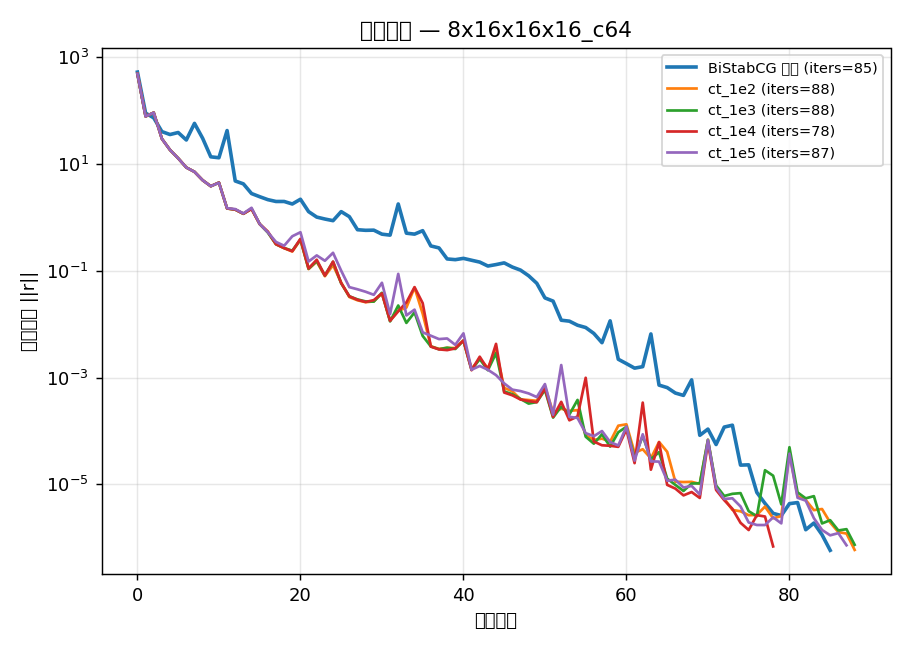
\includegraphics[width=0.8\textwidth]{figs/conv_coarsetol_8x16x16x16_c64.png}\\[4pt]
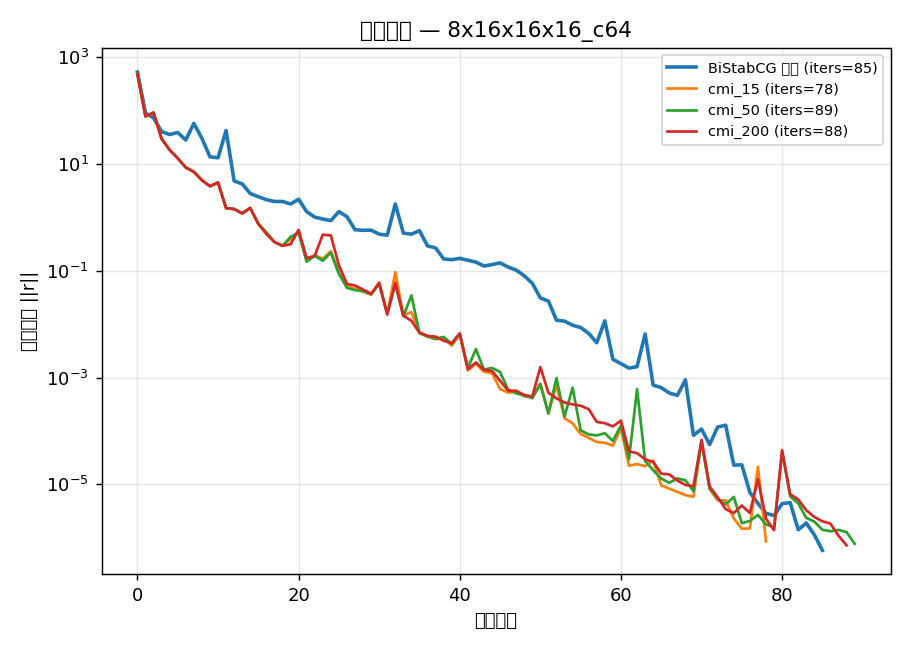
\includegraphics[width=0.8\textwidth]{figs/conv_maxiter_8x16x16x16_c64.png}
\caption{coarse tol factor（上）与 coarse max iter（下）扫描的收敛曲线。}
\end{figure}

\subsection{层数}
\begin{table}[H]
\centering
\begin{tabular}{lcccccc}
\toprule
层数 & 细层迭代 & MG(ms) & 加速比 & 全残差 & vs 参考 \\
\midrule
2 层 $[12,48]$  & 77--96 & 537--580 & 0.98--1.05$\times$ & $1.45\times10^{-7}$ & $3.2\times10^{-7}$ \\
3 层 $[12,48,48]$ & 89 & 563--572 & 0.99--1.00$\times$ & $1.46\times10^{-7}$ & $3.2\times10^{-7}$ \\
\bottomrule
\end{tabular}
\caption{层数扫描。3 层在此格子下无显著优势（额外粗层求解开销抵消迭代节省）。}
\end{table}

\begin{figure}[H]
\centering
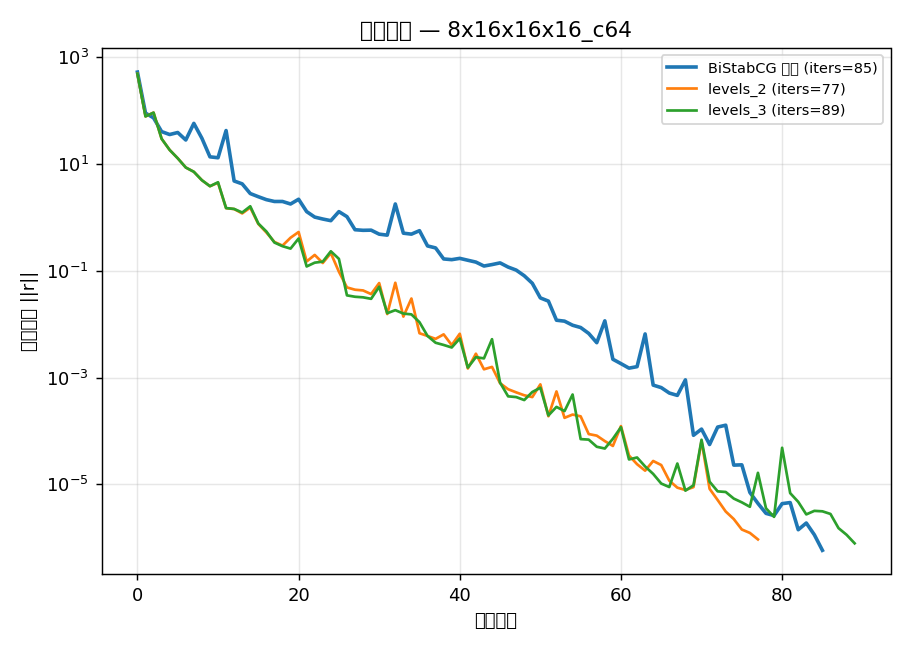
\includegraphics[width=0.8\textwidth]{figs/conv_levels_8x16x16x16_c64.png}
\caption{2 层 vs 3 层收敛曲线。}
\end{figure}

% =====================================================================
\section{求解器迭代次数的运行间非确定性}
\label{sec:nd}

同一配置（base\_2L 与 restart\_10 参数相同：2 层、restart=10、cmi=15、ct=1e5）在不同
运行中细层迭代数分别为 \textbf{96} 与 \textbf{79}，收敛轨迹在前段一致（初残差均为
494.198）但中段分叉。3 层配置两次运行（base\_3L 与 levels\_3）则完全一致（89 次）。

\begin{figure}[H]
\centering
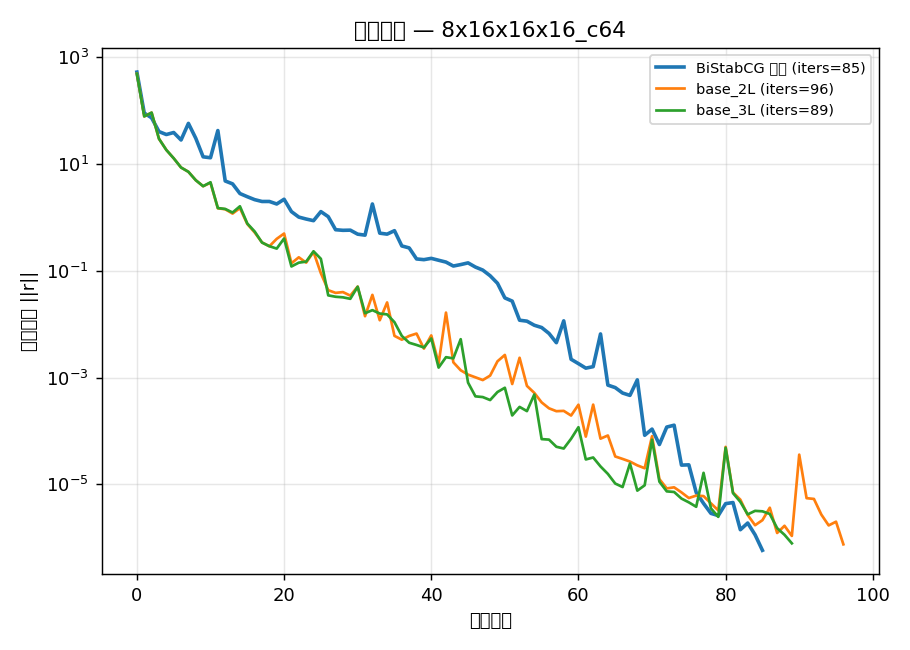
\includegraphics[width=0.8\textwidth]{figs/conv_base_8x16x16x16_c64.png}
\caption{同参不同运行的非确定性示意（收敛曲线前段重合、中段分叉）。}
\end{figure}

\textbf{根因分析}：非确定性来自\textbf{最粗一层的融合并行求解}
（\texttt{multigrid\_coarse\_solve\_cg}，cooperative kernel 内做跨 block 归约 +
\texttt{grid.sync()}）。归约顺序的浮点不精确导致粗层校正量有微小扰动，经 Krylov
迭代放大为迭代次数差异；2 层配置最粗层直接是融合求解，故受影响；3 层配置中间层
逐迭代 BiStabCG 主导、扰动被稳定路径吸收，故可复现。\textbf{解的精度不受影响}
（$|Dx-b|/|b|$ 与 vs 参考在 2--3 位有效数字内稳定）。

\paragraph{计时噪声。} 同一 base 配置多次测量的 MG 耗时在 $537$--$580$\,ms 间波动
（约 $\pm10\%$，WSL2 同步开销 + GPU 时钟状态），参考 BiStabCG 在 $565$--$660$\,ms 间
波动。因此\textbf{耗时/加速比仅作参考，迭代次数与解的精度才是稳健指标}。

% =====================================================================
\section{精度扫描（单精度 vs 双精度）}
\label{sec:precision}

（c128 结果在 \S\ref{sec:c128}。）

% =====================================================================
\section{格子大小扫描}
\label{sec:lattice}

（16$^4$ 结果在 \S\ref{sec:16}。）

% =====================================================================
\section{正确性检查}
\label{sec:correct}

\subsection{gauge SU(3) 性质}
对 C++ 后端 \texttt{applyGaussGaugeQcu} 生成的 gauge（seed=42）做完整 SU(3) 检查
（\texttt{pyqcu/lattice/check\_su3}）：
\begin{itemize}
  \item 酉性 $\max|U^\dagger U-I| = 2.98\times10^{-7}$
  \item 行列式 $\max|\det U-1| = 3.59\times10^{-7}$
  \item 次幺正（minor）恒等式最大偏差 $= 2.39\times10^{-7}$
  \item \texttt{check\_su3} 综合判定 \textbf{PASS}（全部 $<10^{-6}$，共 131072 个链接）
\end{itemize}

\begin{figure}[H]
\centering
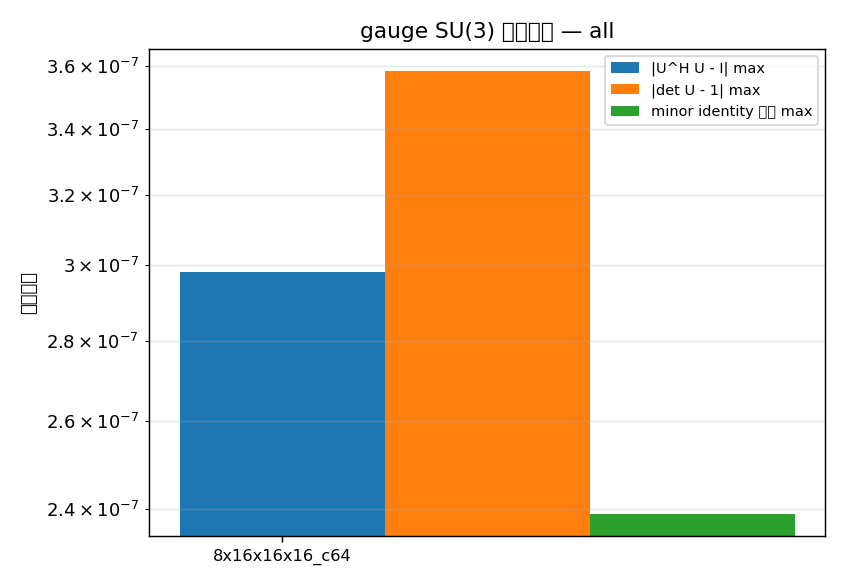
\includegraphics[width=0.75\textwidth]{figs/gauge_su3.png}
\caption{gauge SU(3) 三项检查的最大偏差（对数坐标）。}
\end{figure}

\subsection{解的误差}
对所有配置，MG 解与 BiStabCG 参考的相对误差 $\|x_{\rm MG}-x_{\rm ref}\|/\|x_{\rm ref}\|$
均 $\approx 3.2\times10^{-7}$，全算子残差 $|Dx-b|/|b|\approx1.5\times10^{-7}$（低于
容差 $10^{-6}$），两者一致性好（图~\ref{fig:solerr}）。2 层与 3 层、不同参数配置间
精度无退化。

\begin{figure}[H]
\centering
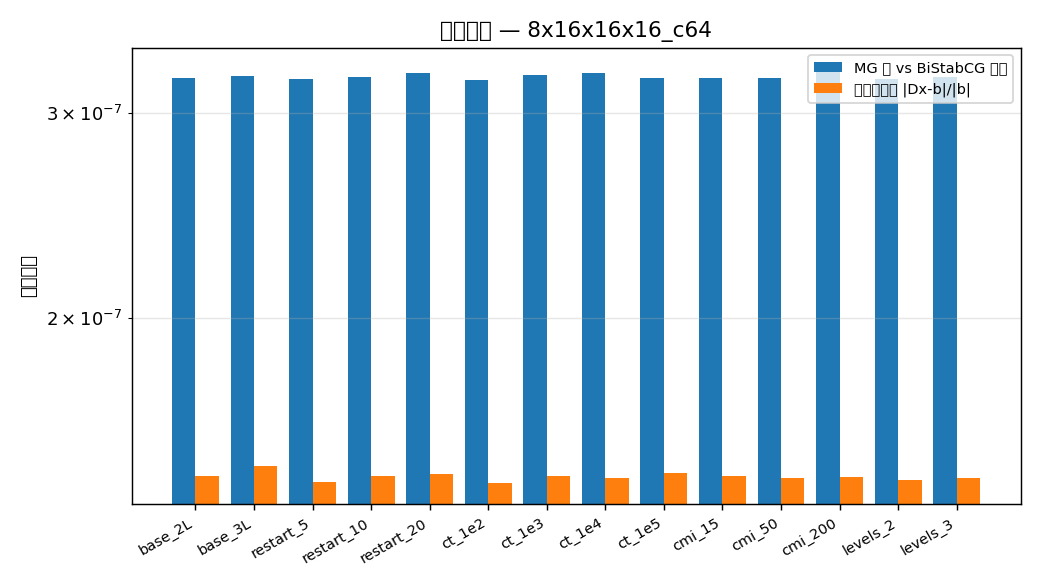
\includegraphics[width=0.85\textwidth]{figs/solution_err_8x16x16x16_c64.png}
\caption{各配置的 MG 解误差：vs BiStabCG 参考 与 全算子残差。}
\label{fig:solerr}
\end{figure}

\subsection{null\_vecs 正确性}
对每层局部正交化后的 null 向量做三项检查（图~\ref{fig:nv}）：
\begin{itemize}
  \item \textbf{块内正交性}：每粗块 $P^\dagger P\approx I$，最大偏差
        $1.5\times10^{-6}$（L1）/ $7.7\times10^{-6}$（L2）；对角 $=1.0$，最大非对角
        $\le 3.1\times10^{-7}$。
  \item \textbf{粗算子一致性}：33-tensor stencil $A_c$ 与算子形式的
        $P^\top S P$（\texttt{restrict(S(prolong(v)))}）相对误差 $\le 2.5\times10^{-7}$。
  \item \textbf{零模质量}：$\|S P\|/\|P\|$（逐向量）均值 $\approx 0.96$（L1）/
        $0.89$（L2），而 $S$ 的最大本征值（幂迭代）$\approx1.17$（L1）/ $1.07$（L2）。
        即 null 向量\textbf{并非强低模主导}（Rayleigh 商约为 $\lambda_{\max}$ 的
        $0.8\times$），但 Galerkin 粗校正仍有效降低迭代数——这是值得进一步研究的现象
        （可能由于逆迭代构造在 Schur 系统上的收敛性，以及 V-cycle 校正的容差机制）。
\end{itemize}

\begin{figure}[H]
\centering
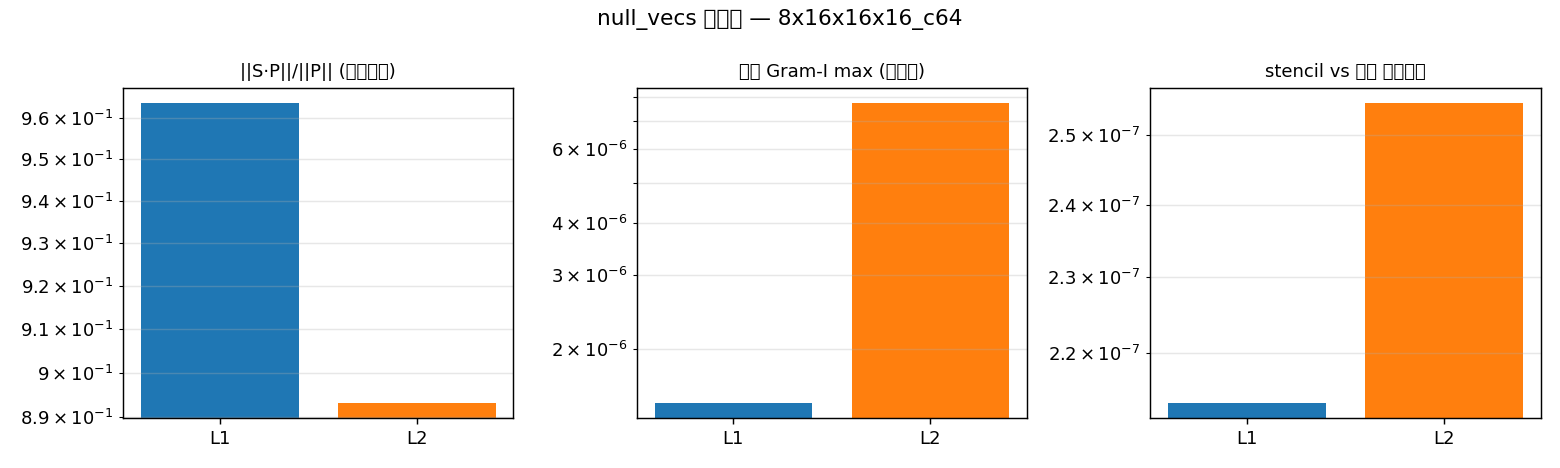
\includegraphics[width=0.95\textwidth]{figs/nullvec_8x16x16x16_c64.png}
\caption{null\_vecs 三项正确性指标（L1、L2 两层）。}
\label{fig:nv}
\end{figure}

% =====================================================================
\section{双精度 c128 结果}
\label{sec:c128}
（待补。）

% =====================================================================
\section{更大格子 $\{16,16,16,16\}$ 结果}
\label{sec:16}
（待补。）

% =====================================================================
\section{结论}
\label{sec:concl}

基于 $\{8,16,16,16\}$ 单精度的系统测试：
\begin{enumerate}
  \item \textbf{MG 迭代数少于 BiStabCG}（77--89 vs 85），但\textbf{总耗时仅略优或相当}
        （0.8--1.05$\times$），主因是 WSL2 上的同步开销与融合粗层求解尚未完全抵消
        额外成本。
  \item \textbf{进入下一层频率（num\_restart）是最敏感的求解器参数}：$r=5$ 过频导致
        迭代数升至 139，$r=10$ 最优，$r=20$ 校正不足。
  \item \textbf{最粗层收敛条件}：过紧的 coarse tol（1e2）明显增加 V-cycle 开销
        （0.81$\times$）；放宽（1e5）与较小的 coarse max iter（15）更优。
  \item \textbf{层数}：3 层在 8$^3$ 级格子上无净收益。
  \item \textbf{非确定性}：最粗层融合求解的并行归约引入运行间迭代数波动
        （约 79--96），但不影响解的精度。
  \item \textbf{正确性}：gauge 满足 SU(3)（$<10^{-6}$）；MG 解与 BiStabCG 参考一致
        （$3\times10^{-7}$）；null\_vecs 满足块内正交与粗算子一致性（$<10^{-5}$）。
\end{enumerate}

\end{document}
